This chapter presents the experiments. It is a crucial part of the thesis and has to dominate in the thesis. 
The experiments and their analysis should be done in the way commonly accepted in the scientific community (eg. benchmark datasets, cross validation of elaborated results, reproducibility and replicability of tests etc).

\section{Methodology}

\begin{itemize}
\item description of methodology of experiments
\item description of experimental framework (description of user interface of research applications – move to an appendix)
\end{itemize}

\subsection{Time execution}

\subsection{Image compression}


\section{Data sets}

The image data set gathered to evaluate results of the thesis takes its origin from one of
Tilo Strutz's papers \cite{ref_images}. It was used at first to evaluate multiplierless reversible
color transforms. The main purpose of that paper was to propose an entire family of multiplierless
reversible color transforms and investigate their performance in lossless image compression \cite{multiplierless_rct}.
Therefore it was found out to be suitable for the case of this thesis as lossless image compression
on color pictures is applied as well. The examplary elements of the image data set are available at
figures \ref{fig:example_1}, \ref{fig:example_2} and \ref{fig:example_3}. It is worth noticing that only ppm
(portable PixMap) images were selected due to lack of png format support in Kakadu library.

\begin{figure}
    \centering
    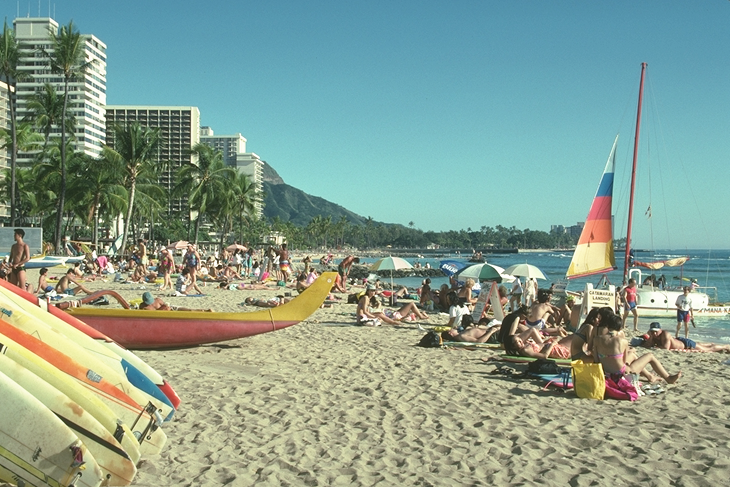
\includegraphics[scale=0.5]{384007.png}
    \caption{The example image from the reference data set \cite{ref_images}}
    \label{fig:example_1}
\end{figure}

\begin{figure}
    \centering
    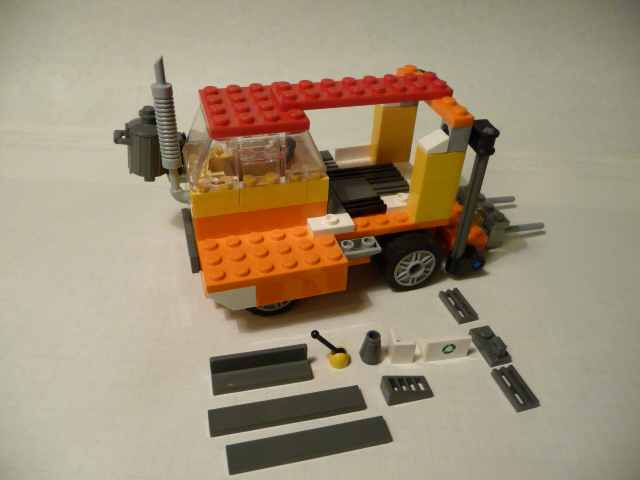
\includegraphics[scale=0.5]{im_0069.png}
    \caption{The example image from the reference data set \cite{ref_images}}
    \label{fig:example_2}
\end{figure}

\begin{figure}
    \centering
    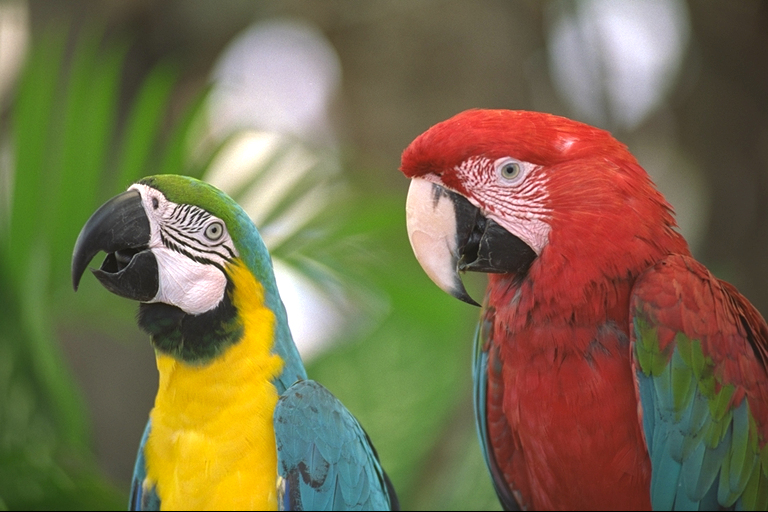
\includegraphics[scale=0.4]{kodim23.png}
    \caption{The example image from the reference data set \cite{ref_images}}
    \label{fig:example_3}
\end{figure}


\section{Results}

\begin{itemize}
	\item presentation of results, analysis and wide discussion of elaborated results, conclusions
\end{itemize}

\subsection{Reference results}

\subsection{Estimated best configuration}

\subsection{Comparison with reference}

\subsection{Time comparison}

\subsection{Visualized sample results}

There are presentend sample outputs of various dwt variants applied to famous 512x512 picture
of Lena Forsén \cite{lena}. All the images are results of low-pass filtering from the last
rank of discrete wavelet transform. The first image \ref{fig:lena_dwt_5} represents the Part 2
compatible decomposition variant where transformation is applied each time only to columns.
Therefore the shape of result is very thin rectangle. Second picture \ref{fig:lena_dwt_199}
illustrates mainly row-wised based dwt.
Another figure \ref{fig:lena_dwt_326} depicts mixed version of discrete wavelet transform described
before. Last one \ref{fig:lena_dwt_363} is the output of Part 1 compliant decomposition.

\begin{figure}
    \centering
    
\includegraphics[scale=0.5]{lena_dwt_5.png}
    \caption{The example output image of dwt processing chain using Lena test image \cite{lena}}
    \label{fig:lena_dwt_5}
\end{figure}

\begin{figure}
    \centering
    
\includegraphics[scale=1]{lena_dwt_199.png}
    \caption{The example output image of dwt processing chain using Lena test image \cite{lena}}
    \label{fig:lena_dwt_199}
\end{figure}

\begin{figure}
    \centering
    
\includegraphics[scale=1]{lena_dwt_326.png}
    \caption{The example output image of dwt processing chain using Lena test image \cite{lena}}
    \label{fig:lena_dwt_326}
\end{figure}

\begin{figure}
    \centering
    
\includegraphics[scale=1]{lena_dwt_363.png}
    \caption{The example output image of dwt processing chain using Lena test image \cite{lena}}
    \label{fig:lena_dwt_363}
\end{figure}
